\section{Durchführung}
\label{sec:Durchführung}
Der Versuchsaufbau ist schematisch in Abbildung (\ref{fig:allgemeiner_Versuchsaufbau}) zu sehen. 
\begin{figure}
    \centering
    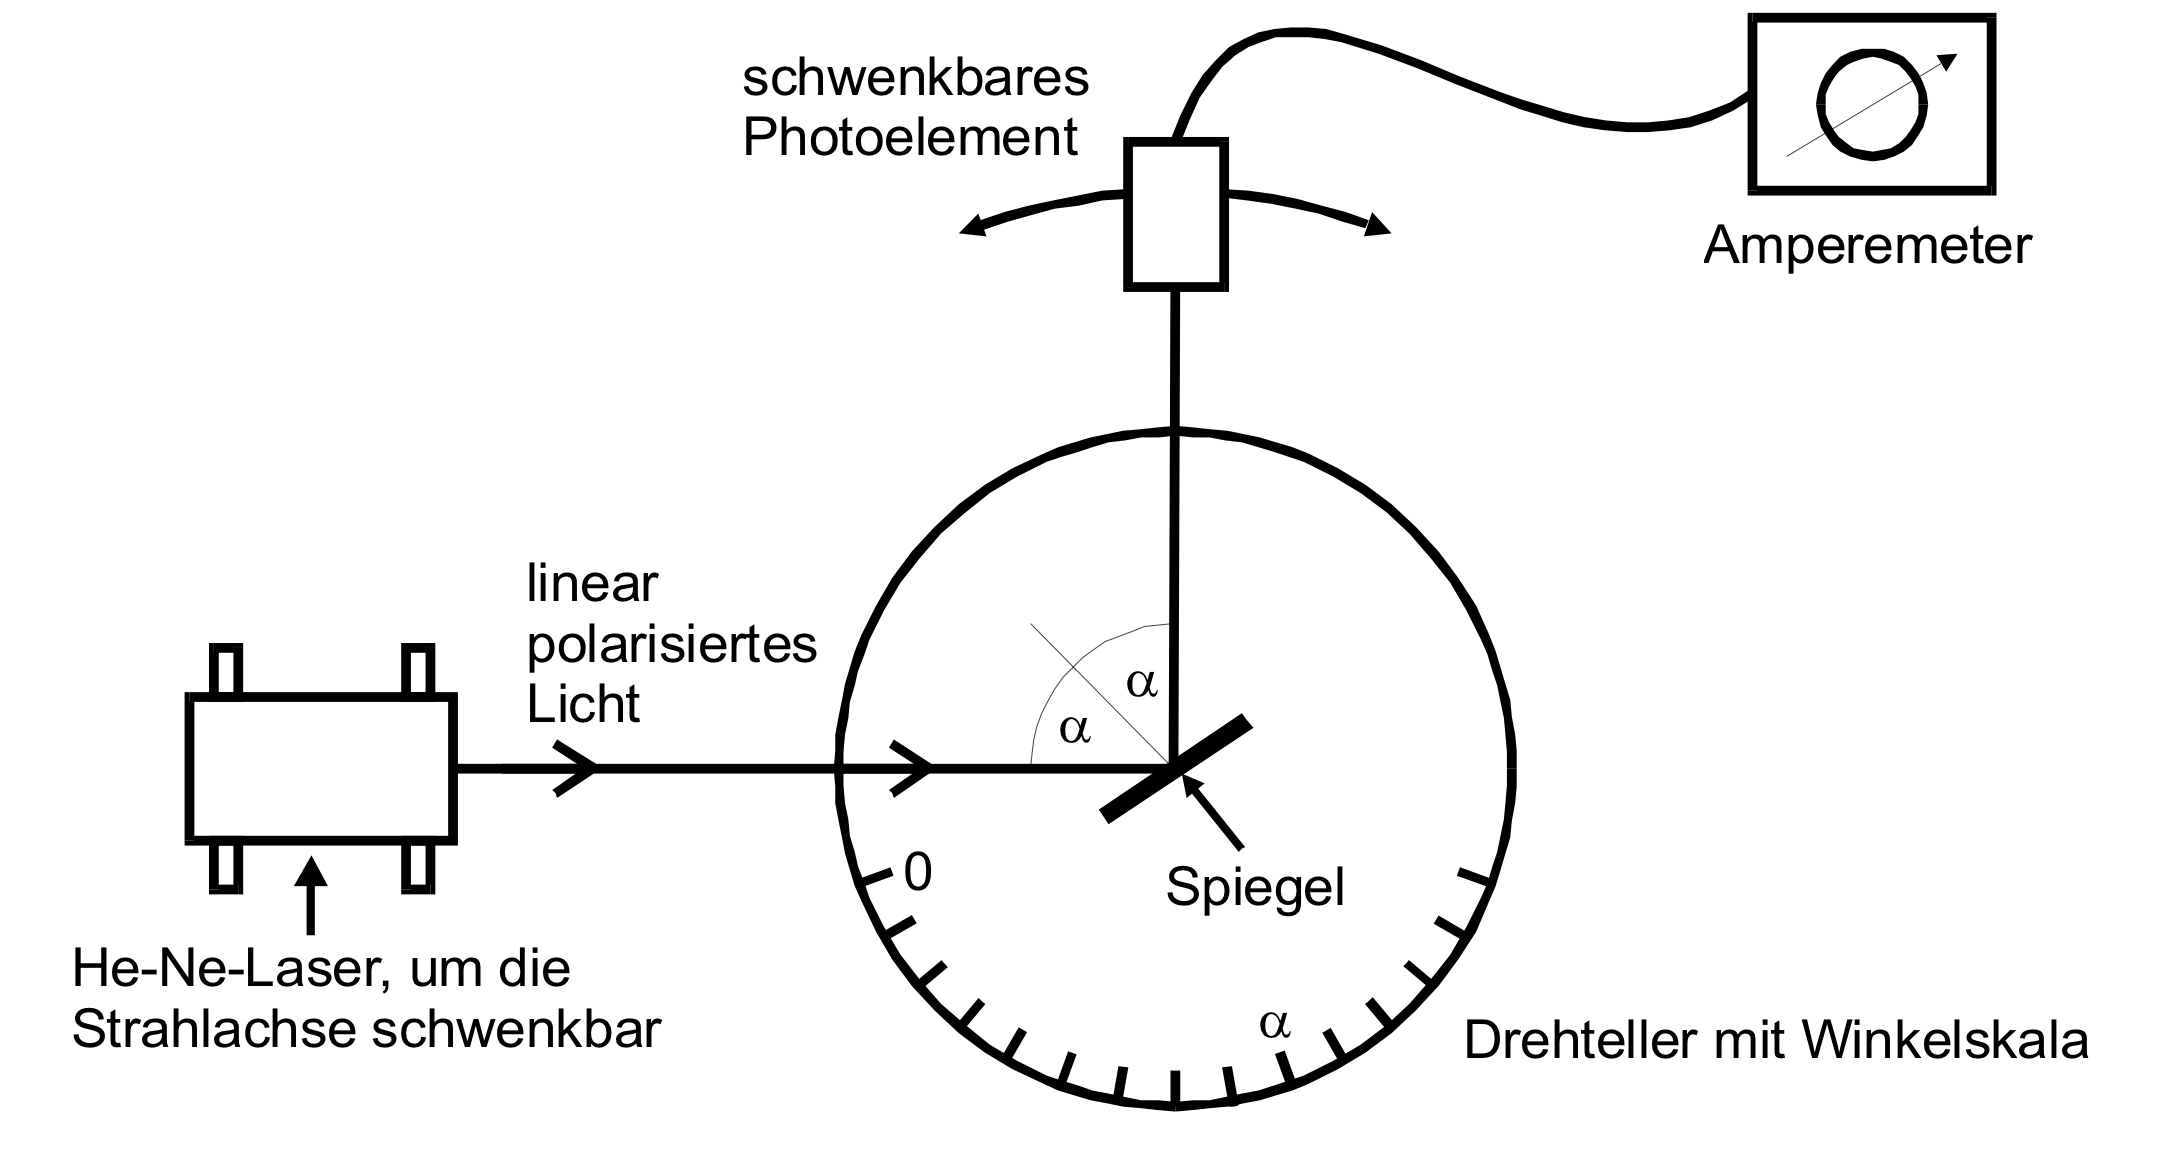
\includegraphics[width=0.8\textwidth]{content/Bilder/Versuchsaufbau_allgemein.jpeg}
    \caption{Schematische Darstellung eines in der Einfallebene schwindeneden Lichtstrahls. Q\cite{anleitungV407}}
    \label{fig:allgemeiner_Versuchsaufbau}
\end{figure}
Der Versuch besteht aus einem Laser einem drehbaren Spiegel aus Silizium und einem Goniometer. Mit diesem kann die Lichtintensität in Ampere gemessen werden. 
Zu Beginn wird der Laser so eingestellt, dass der Strahl auf dem Spiegel auf gleicher Höhe reflektiert wird. Der Spiegel steht dabei senkrecht zum 
Laser. Danach wird eine Dunkelstrommessung durchgeführt, die 
die Intensität der Umgebungshelligkeit bestimmt. Dazu wird der Laser ausgeschaltet. 
Danach wird in einem Bereich von ungefähr 5° bis 70° in 2° Schritten der Spiegel rotiert und die Intensität des refektierenden Laserstrahls gemessen. Ab 70° wird ein 
1° Schritten die Messung fortgeführt bis der Spiegel um 80° gedreht ist. Im Anschluss wird in 2° Schritten bis mindestens 86° weitergemessen. 